\section{What is Percolation Theory?}
Graphs are a fundamental part of nature, therefore the study of them is of great importance in a number of different fields.
A graph can be anything from a random network composed of points (nodes) and connections (edges) between them to a lattice or set of points in a periodic arrangement.
To study such things we need a framework in which to do so; this is where percolation theory enter the picture.
Percolation theory is in the intersection of multiple other topics such as graph theory, probability theory, and statistical physics, combining them in a way to give us the tools we need to study how groups (clusters) of points behave and evolve within a a network or structure.
Percolation can be observed in a variety of environments ranging from the spread of a forest fire to the dissemination of information across a communications network.
We often use percolation theory in physics to help us model how something dissipates or flows through a system, e.g. the electrical conductivity or porousness of a material.
Some of the applications outside of physics include testing the durability of a transportation infrastructure or determining to what extent a product or idea might be adopted by society.
Percolation theory is a broad subject with the ability to be applied to problems in many different disciplines \cite{intro_to_percolation_theory} \cite{applications_of_percolation_theory}.

To get a better understanding of what percolation is, let us discuss a few examples.
Society is developing faster than ever before due to the propagation of information and goods through networks we have constructed.
These networks then allow us to create and participate in increasingly more advanced networks, thus it is critical that we study and understand how these networks behave so that we can get an idea of how to manage and improve them.
The most well known being the internet, which sustains a massive flow of information between billions of people across the globe.
When something is posted online one might ask: how many people will it reach?
To answer this one would start at the source node then see which nodes it could possibly be connected to.
If each person has a probability $p$ of sharing it with another person then we can construct a probabilistic model to determine what the cluster could possibly look like.
If the probability is high then we would expect the size of cluster to be of significant size when compared to the size of the whole network.

Another interesting application is that to the spread of health epidemics across a population.
If there is a virus going around there is an underlying network that can be studied; there is the initial person(s) who contracted the virus and then the people who were contaminated from coming in contact with those infected.
Thus the obvious question is: how much of the population will it affect?
Let us say in a very basic sense that an infected person has a $p$ percent chance of infecting those they come into contact with.
If the virus is treatable and $p$ is low, then we would expect the virus to be eradicated fairly quickly since doctors have the time and ability to treat the outbreak properly.
On the other hand if $p$ is high, say higher than some critical probability $p_c$, then we might expect a different scenario where the virus spreads across the population, i.e. percolates, much like the Ebola epidemic in West Africa during 2013-2016.
Therefore, percolation theory plays a crucial role in helping us answer important questions when it comes to determining how something might spread or propagate across a network or structure.









\subsection{Phase Transitions}
To understand the most important use of percolation theory we must first understand what a phase transition is.
In physics we often encounter systems which have different properties depending on which phase they're in.
Thus we are interested in how the system behaves around the critical point.
A phase transition is usually characterized by an order parameter, which is a variable that is zero in one phase and non-zero in the other, giving us the ability to distinguish phases and identify phase transitions.

In percolation theory we define the order parameter as the ratio of the largest cluster to the size of the system, i.e. if we have $n$ nodes total and the largest cluster $C$ contains $|C|$ nodes, then the order parameter $P$ is given by:

\begin{equation}
	\label{eqn:order_parameter}
	P := \frac{|C|}{n}
\end{equation}
Of course the system is usually examined in the thermodynamic limit ($n \rightarrow \infty$), thus $P$ is zero unless there exists a macroscopic cluster.

There are two main types of phase transitions: first- and second-order.
In a first-order phase transition there is what we call a latent heat, i.e. energy that is either absorbed or emitted during a process where the temperature is fixed, e.g. the transition of water between the solid and liquid phases.
Second-order (also called continuous) phase transitions are characterized by a divergent correlation length and power law behavior of variables which leads to a set of critical exponents (more about critical exponents below).
The reason they are called continuous transitions is because the order change in the order parameter at the critical point is continuous.
The classic percolation models are known to undergo continuous phase transitions, making them useful for modeling such systems.









\subsubsection{Critical Exponents}
Around the critical point in a percolation model, there exists a set of numbers called the critical exponents which contain information about how certain quantities of interest behave.
Let's take for example the order parameter as a function of the occupation probability $p$, which is described by the critical exponent $\beta$ \cite{intro_to_percolation_theory}:

\begin{equation}
	\label{eqn:crit_exp_P}
	P(p) \sim (p - p_c)^\beta
\end{equation}
The average cluster size $\langle s \rangle$ is described by $\gamma$ \cite{intro_to_percolation_theory}:

\begin{equation}
	\label{eqn:crit_exp_s}
	\langle s \rangle (p) \sim (p - p_c)^{-\gamma}
\end{equation}
The correlation length $\xi$ is described by $\nu$ \cite{intro_to_percolation_theory}:
\begin{equation}
	\label{eqn:crit_exp_xi}
	\xi (p) \sim |p - p_c|^{-\nu}
\end{equation}

The neat thing about these exponents is that they are universal in the sense that they only depend on the dimension $d$ of the system, regardless of the microscopic configuration.
Some values for these are given in the table below \cite{intro_to_percolation_theory}:

\begin{center}
  \begin{tabular}{ | l | c | c | c | }
    \hline
    $d$ & $\beta$ & $\gamma$ & $\nu$ \\ \hline
    2 & 5/36 & 43/18 & 4/3 \\ \hline
    3 & 0.41 & 1.82 & 0.88 \\
    \hline
  \end{tabular}
\end{center}









\subsection{Percolation on a Lattice}
On a lattice we can look at percolation from two different perspectives: site and bond percolation.
With site percolation we study graphs where the sites of a lattice are either occupied or unoccupied, whereas with bond percolation we study the graphs where the connections between sites are either active or inactive.
The underlying concepts of percolation are the same, but in practice the details differ slightly.



\subsubsection{Site Percolation}
For this we consider a lattice of dimension $d$.
Let us take our lattice to be hyper-cubic with side length $L$, giving us a total of $L^d$ sites in the lattice.
We then occupy each site of the lattice with probability $p$ (unoccupied with probability $1 - p$), independent of all other sites.
We can then use indicator random variables $X_1, ..., X_{L^d}$ to represent if the sites are occupied or not, where:

\[
X_i =
\begin{cases}
	1 & \text{if site } i \text{ occupied} \\
	0 & \text{otherwise}
\end{cases}
\]

The number of occupied sites in the lattice is then given by $\sum_i X_i$, which is expected to be $L^d p$.
The notion of a cluster $I = \{i_1, ..., i_s\}$ of size $s = \sum_{i \in I} X_i$ is defined as a set of $s$ occupied sites which are nearest neighbors with at least one other site in the set.
If we let $N_s$ represent the number of clusters of size $s$, and $n_s = N_s / L^d$, then we can also look at the probability that any given site is part of a cluster:

\begin{equation}
	\label{eqn:p_in_cluster}
	\sum_s s n_s
\end{equation}

This now gives us the ability to determine the probability that the given site is part of a cluster of size $s$:

\begin{equation}
	\label{eqn:p_in_cluster_size_s}
	\frac{s n_s}{\sum_{s'} s' n_s'}
\end{equation}

Using the above we can now compute the average cluster size:

\begin{equation}
	\label{eqn:avg_cluster_size}
	\langle s \rangle = \sum_s s \frac{s n_s}{\sum_{s'} s' n_s'}
\end{equation}

Thus it is clear that we can obtain a significant amount of information by applying basic probability theory.
Now that we have defined clusters and cluster sizes we can talk about the idea of a percolating cluster.
This is a cluster which spans from one side of the lattice to the opposite in any of the $d$ dimensions.
It's obvious that the presence of a percolating cluster is heavily dependent on $p$, since for low $p$ we wouldn't expect to see a cluster spanning across the lattice.
However, this is also dependent on $L$, and we often seek to study the limiting case where $L \rightarrow \infty$.
This leads us to the concept of a critical probability, $p_c$, such that when $p > p_c$ we expect to see a percolating cluster, but not when $p < p_c$.

\paragraph{One-Dimension}
We now consider the simplest case where $d = 1$, which allows us to analytically solve for some quantities of interest.
Fig. \ref{fig:1d_site_clusters} illustrates a snippet of an infinite 1D lattice where the solid black sites are active and the white ones are inactive.
There are a total of four clusters visible (highlighted in blue): two one-clusters, a three-cluster, and a four-cluster.

\begin{figure}[H]
	\centering
	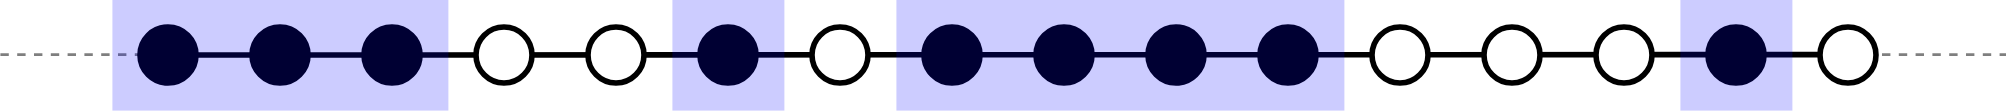
\includegraphics[width=350pt]{images/1d-site-clusters.png}
	\caption{1D Site Clusters}
	\label{fig:1d_site_clusters}
\end{figure}

For comparison Fig. \ref{fig:1d_bond_clusters} illustrates a 1D lattice where all sites are active and only some of the bonds between them are active.
There are a total of four clusters visible (highlighted in blue): two two-clusters, a three-cluster, and a four-cluster.

\begin{figure}[H]
	\centering
	\includegraphics[width=350pt]{images/1d-bond-clusters.png}
	\caption{1D Bond Clusters}
	\label{fig:1d_bond_clusters}
\end{figure}

The probability that any given site is part of a cluster of size $s$ is then given by the product of the independent probabilities of the site to the left of the leftmost site in the cluster being unoccupied, $s$ consecutive sites being occupied, and the site to the right of the rightmost site in the cluster being unoccupied, i.e.:

\begin{equation}
	\label{eqn:n_s_1d}
	n_s = (1 - p) \cdot p^s \cdot (1 - p) = p^s (1 - p)^2
\end{equation}

Plugging Eq. \ref{eqn:n_s_1d} into Eq. \ref{eqn:p_in_cluster} we find:

\begin{equation}
\begin{split}
	\sum_s n_s s &= (1 - p)^2 \sum_s s p^s\\
	&= (1 - p)^2 p \frac{d}{dp} \sum_s p^s\\
	&= (1 - p)^2 p \frac{d}{dp} \frac{p}{1-p}\\
	&= (1 - p)^2 p \bigg[ \frac{1}{1-p} + \frac{p}{(1 - p)^2} \bigg]\\
	&= p
\end{split}
\end{equation}

Where the second equality is obtained by linearity of the derivative and summation operators and realizing that $s p^s = p \frac{d}{dp} p^s$, the third by noticing that $\sum_s p^s$ is the power series for $\frac{p}{1-p}$, the fourth by application of the derivative operator, and the final by algebaic manipulation.
Therefore there is a $p$ percent chance that any given site is part of a cluster, which when thought about is fairly obvious.
Using the above we can also analytically determine the average cluster size (again using the trick of differentiating $p^s$ to bring down an $s$):

\begin{equation}
\begin{split}
	\langle s \rangle &= \sum_s \frac{s^2 n_s}{\sum_{s'} s' n_s'}\\
	&= \frac{(1 - p)^2}{p} \sum_s s^2 p^s\\
	&= \frac{(1 - p)^2}{p} \bigg[p\frac{d}{dp}\bigg]^2 \sum_s p^s\\
	&= \frac{(1 - p)^2}{p} \bigg[p\frac{d}{dp}\bigg]^2 \frac{p}{1 - p}\\
	&= \frac{(1 - p)^2}{p} p \frac{d}{dp} \bigg[ \frac{p}{1-p} + \frac{p^2}{(1 - p)^2} \bigg]\\
	&= \frac{1 + p}{1 - p}
\end{split}
\end{equation}

The above illustrates that we can analytically solve for some of the above quantities of interest in the one-dimensional case.
We're often more interested in the thermodynamic limit, that is for systems that is, when $L \rightarrow \infty$.
In the thermodynamic limit, percolation on the chain only occurs when we have an infinite number of neighboring occupied sites.
This means that if just one site out of the entire chain is unoccupied there is no percolating cluster, which leads us to conclude that for the one-dimensional case $p_c = 1$.

\paragraph{Multiple-Dimensions}
Unfortunately it is not as straight forward in higher dimensions due to the many different arrangements and shapes that the clusters can take on.
This is illustrated in Fig. \ref{fig:2d_site_clusters} where we can see four possible arrangements of a nine-cluster, each with different numbers of neighboring inactive sites.

\begin{figure}[H]
	\centering
	\includegraphics[width=350pt]{images/2d-site-clusters.png}
	\caption{2D Site Clusters}
	\label{fig:2d_site_clusters}
\end{figure}

Therefore, we lose our ability to answer our questions through analytical methods and we must resort to numerical methods and simulations to study the system.
This is where computer simulations and finite-size scaling analysis come in handy.
Due to the limitations of computational power we can only simulate systems up to certain sizes, however, we would still like to know gather some information about the infinite size system.
What we do is we simulate systems of varying sizes and see how the quantities of interest scale with the system size, which gives us the ability to extrapolate to the thermodynamic limit.

\paragraph{Example: Ising Model}
The Ising model is the most well-known model of ferromagnetism, undergoing a second-order phase transition (for $d \ge 2$) from the ordered, ferromagnetic state at low temperatures to the disordered, paramagnetic state at high temperatures.
This model has played a critical role in the development and understanding of statistical physics.
The basic idea is that given a lattice of size $L^d$, at each site $i$ of the lattice there is a spin $\sigma_i$ oriented in either the up or down direction.
The order parameter characterizing the transition is the magnetization $m = \frac{1}{L^d} \sum_i \sigma_i$.
A (simplified) Hamiltonian of the system in the configuration $\{\sigma\}$ is then given by:

\begin{equation}
	\label{eqn:Ising_Hamiltonian}
	H(\{\sigma\}) = -J \sum_{\langle i j \rangle} \sigma_{ij} -h \sum_i \sigma_i
\end{equation}

Where the sum is over all neighboring spin pairs, $J$ is the coupling constant between spins, and $h$ is a mean field per spin approximation.
Using this combined with statistical and computational physics methods we are able to simulate how this system behaves as the size increases.
One useful tool when modeling such a system is the use of periodic boundary conditions, which help reduce the finite-size effects of smaller lattice sizes.
In Fig. \ref{fig:Ising_percolation} we can see a percolating cluster of up (black) spins at the critical temperature $T_c = 2 / \log(1 + \sqrt{2})$ on a 2D square lattice with side-length $L = 128$.
Fig. \ref{fig:Ising_percolation} was generated using the Wolff single cluster algorithm with $5 \cdot 10^4$ update sweeps over the lattice.

\begin{figure}[H]
	\centering
	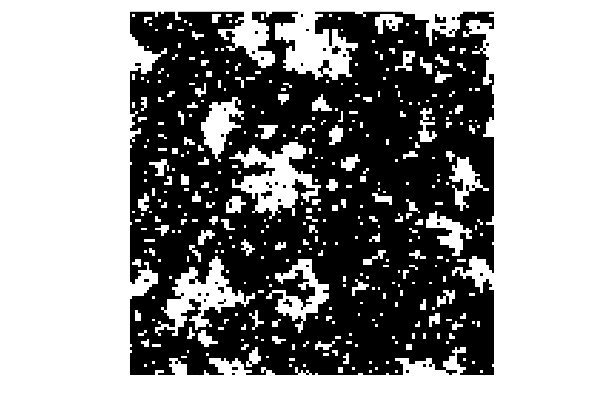
\includegraphics[width=350pt]{images/Ising-128-percolation.png}
	\caption{2D Ising Model Percolating Cluster}
	\label{fig:Ising_percolation}
\end{figure}









\subsection{Percolation on a Network}
Percolation can also be observed on networks, so we will now discuss some of the basic ideas behind network percolation as a segue to the next section.
In the late 1950s and early 1960s Paul Erdős and Alfréd Rényi published several papers on random networks, leading to the creation of what is known today as the Erdős-Rényi model (ER) \cite{ER1} \cite{ER2}.

To get an idea of how it works we imagine a graph starting with a set of $n$ disconnected nodes at $t = 0$, giving us ${n \choose 2}$ possible connections between them.
Then at each step in the evolution process two nodes are chosen at random and connected by an edge, thus after $t$ steps there are a total $t$ edges present in the graph.

A cluster on a random network is a set of nodes connected by edges, either directly or indirectly.
Being that some clusters in the graph will of course merge together over time, there exists an attractive potential of sorts between clusters corresponding to the likelihood that the clusters will merge together to form a larger one.
To demonstrate this let's take three clusters $C_1, C_2,$ and $C_3$ of sizes $|C_1|, |C_2|,$ and $|C_3|$, with $|C_1| > |C_2|$ leaving $|C_3|$ arbitrary.
Then we let $\Phi_1$ ($\Phi_2$) be the potential between the first (second) cluster and the third.
In a graph where each connection is equally probable, the probability that the first or second cluster merges with the third is directly proportional to the size of the cluster because more nodes means more possible connections.
Therefore, there is a higher probability that the first cluster rather than the second merges with the third and we conclude that $\Phi_1 > \Phi_2$.

In the a network, percolation occurs when a giant (macroscopically large) cluster appears.
The order parameter here is defined as the largest cluster size divided by the network size, i.e. $|C| / n$.
Let $n$ be the number of nodes, $t$ be the number of edges present in the graph, and take $r = t/n$.
If $r > 0.5$ then there will exist a percolating cluster within the graph, but not if $r < 0.5$ \cite{ER2}, thus $r = 0.5$ is the critical point where the system transitions from the disconnected state to the state of large scale connectivity.
Letting $|C|$ be the size of the largest cluster, it can be shown that for $r < 0.5$ the largest cluster size scales as $C \sim \log n$, and for $r > 0.5$ $C \sim n$, and more specifically if $r \gtrsim 0.5$ one finds $C \approx (4r - 2)n$ \cite{ER2}.
Therefore, the ER model exhibits a continuous phase transition when the number of edges exceeds half the number of nodes in the graph.
Looking at Fig. \ref{ER_transition} we can see that the order parameter is zero up until $r = 0.5$ when it transitions to the state of large scale connectivity.

\begin{figure}[H]
	\centering
	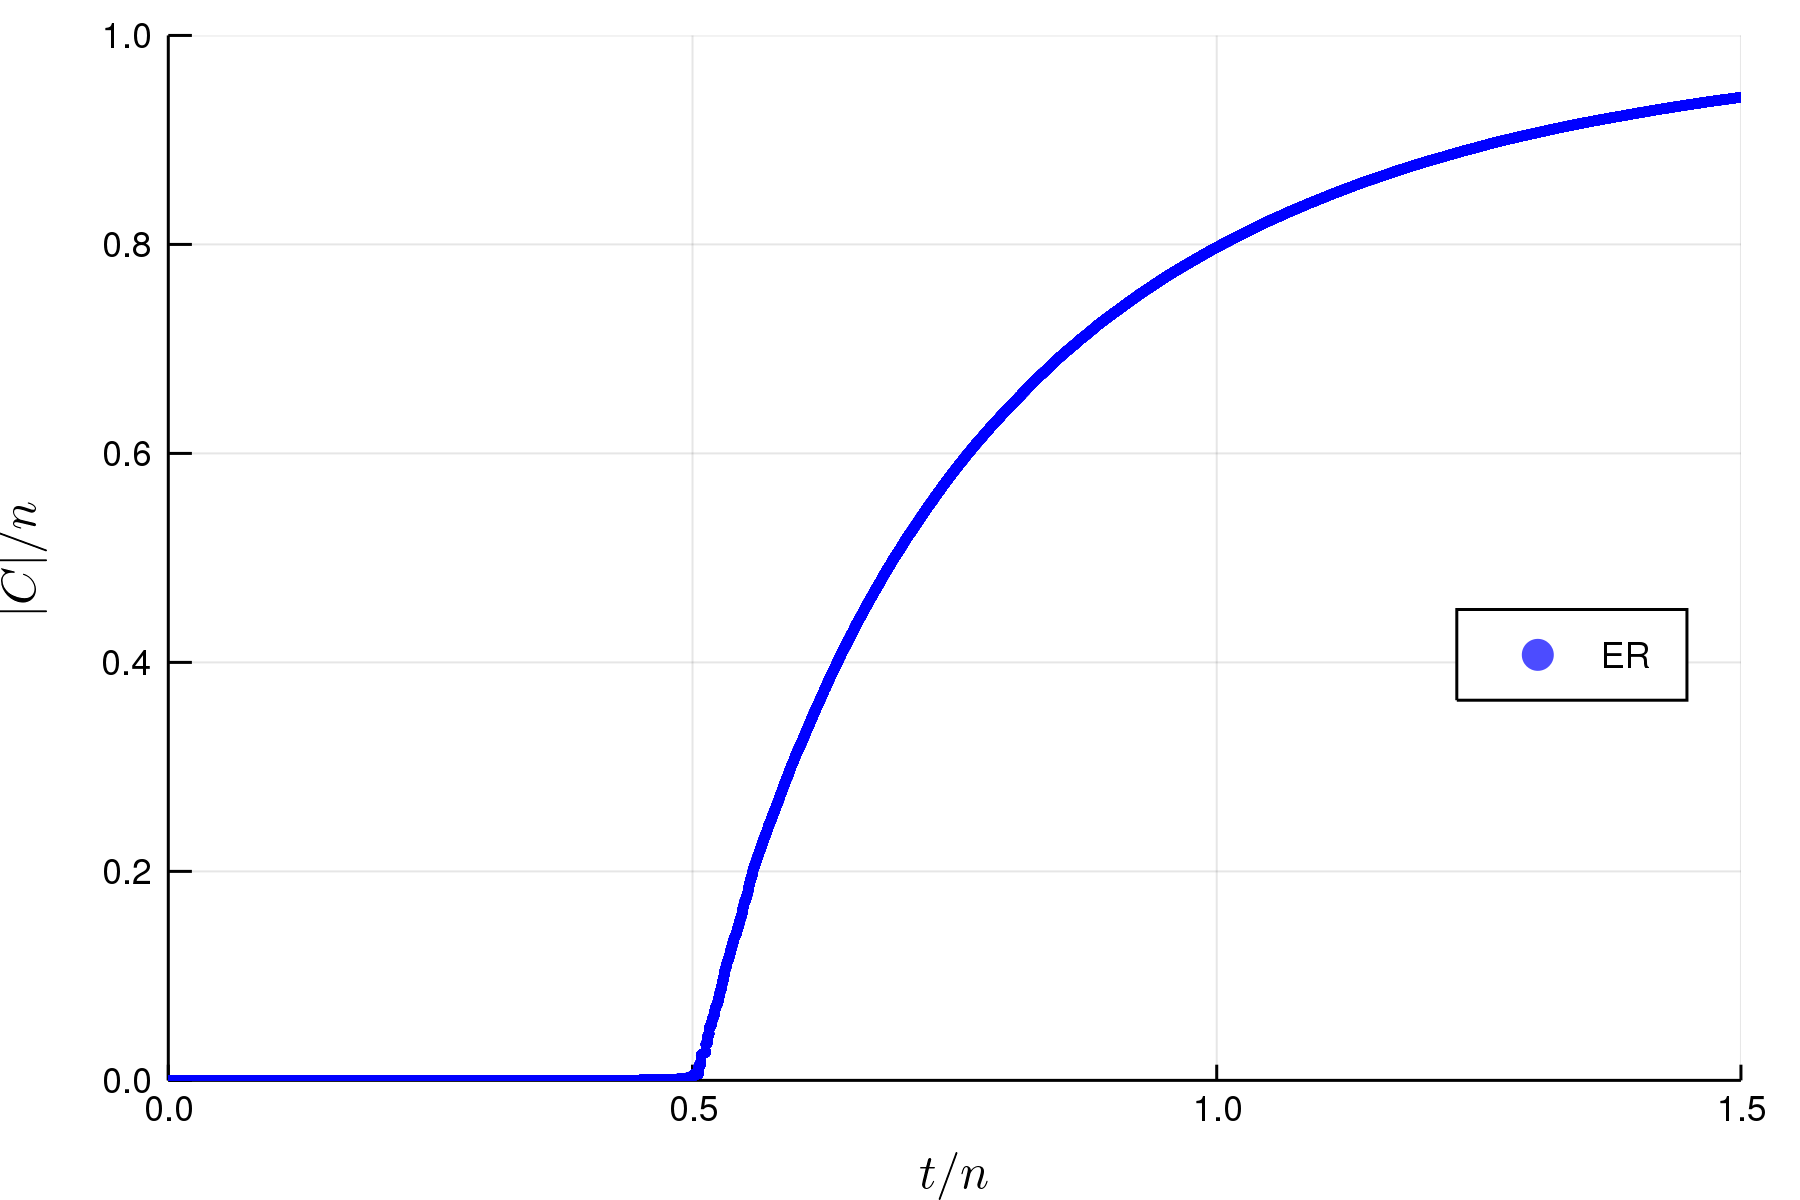
\includegraphics[width=350pt]{images/ER-1e6-order-param.png}
	\caption{Erdős-Rényi Model Order Parameter, $n = 10^6$}
	\label{fig:ER_transition}
\end{figure}
